\chapter{Implementation} \label{implementation}
This chapter will elaborate on the test data used as well as the process that was followed to achieve the results in Chapter \ref{results}.
\section{Existing data}
The data used was acquired by \cite{Westhuyzen:2020} for an article assessing the charring rate of both SA-Pine and Eucalyptus.
	For the purpose of this project, only the data obtained from the SA-Pine test was considered and analysed. 
	\subsection{Summary of test}
	The test was conducted on a sample of 100mm by 0.9m x 0.9m panel of cross-laminated SA-pine.
	This sample was then divided into nine cubes of 100 mm x 100 mm x 100 mm.
	%The sample was a 100 mm by 0.9m x 0.9m panel of cross-laminated SA-pine, this sample was then divided into nine cubes of 100 mm x 100 mm x 100 mm.
	Each cube was fitted with seven Type K-thermocouples placed at consecutive 16.5 mm drilled holes, as can be seen in Figure \ref{TC_layout}. 
	The test panel was tested in a furnace and was exposed to the standard ISO 834 Fire curve \ref{firecurve_fig} on one side and room temperature on the other. 
	The panel was exposed to the fire curve for 50 minutes, at which stage near complete de-lamination was observed and the test ended.
	\begin{figure}[H]
	\centering
	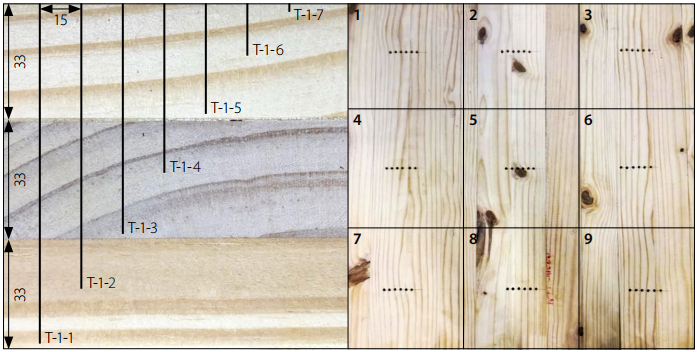
\includegraphics[width=0.75\linewidth]{figures/TC_layout.png}
	\caption{Thermocouple layout in test conducted by \cite{Westhuyzen:2020} cross-section (left) and overall layout (right)}
	\label{TC_layout}
	\end{figure}
	
	\begin{figure}[H]
	\centering 
	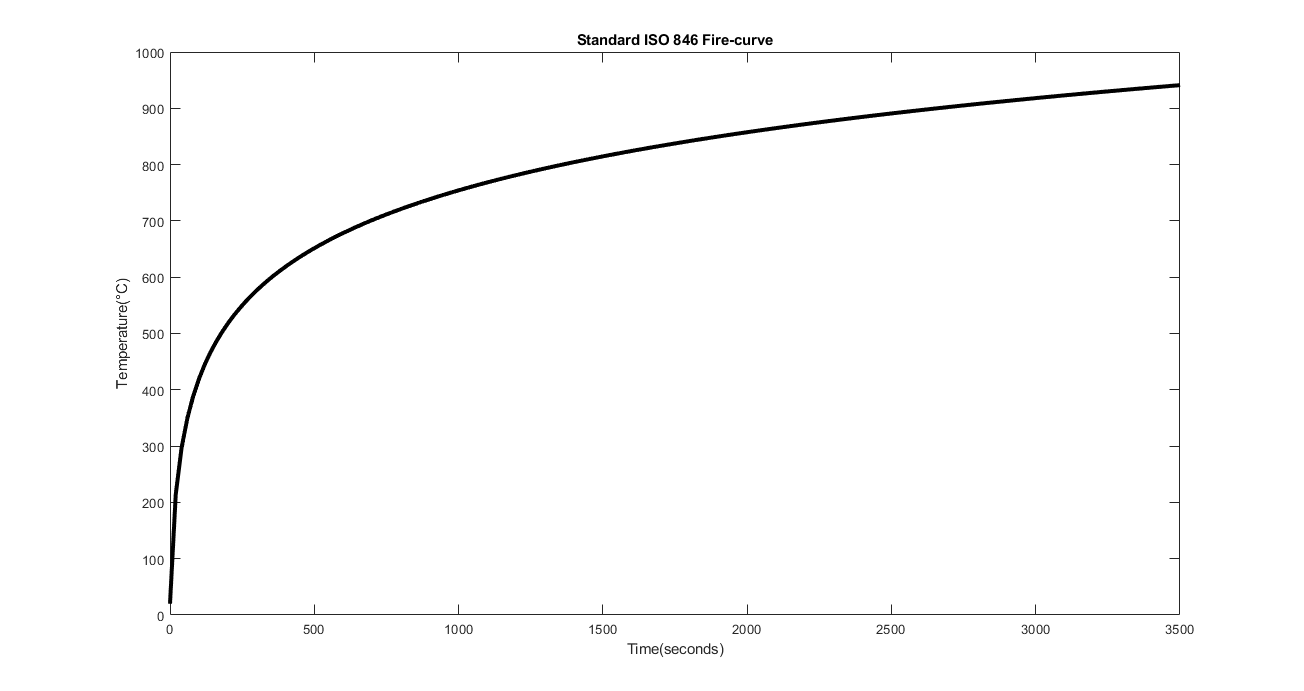
\includegraphics[width=\linewidth]{figures/firecurve.png}
	\caption{Standard ISO fire curve TODO}
	\label{firecurve_fig}
	\end{figure}
	
	\subsection{Potential inaccuracies}
	As with most tests, everything is not always perfect. 
	The potential inaccuracies are discussed below. 
	
	In the data, it was observed that two of the thermocouples broke during testing, this resulted in temperature with a magnitude of $10^{13}$. 
	That temperature is not possible as the highest ever recorded temperature reached was $4\text{x}10^{12}$ and that only occurred in a atomic explosion. %(https://www.insidescience.org/news/hottest-temperature-universe-measured)% 
	This malfunction required that two of the depth measurements were no longer the average between nine samples but instead the average between eight.
	Another inaccuracy that could potentially influence the accuracy of the final result is the accuracy of the depth of the holes in which the thermocouples were placed. 
	%As this was done by hand in the laboratory.
	
	There is also debate about the significance of the contribution of the timber burning to the temperature inside the furnace. 
	For the purposes of this project, it will be assumed that the timber burning does not contribute to the temperature inside the furnace.
	
\section{Finite Element Modelling}\label{femexpl}
A one-dimensional finite element model that simulates what we expect to obtain from the fire tests based on the simplified $kappa$-values provided in EN 1995:1-2-2004 is modified into a function.
This function should provide the temperature of the modelled element based on a specified location and thermal conductivity.
The derivation and adaptation of the model are expanded on below.
	\subsection{Derivation}%"CREATION?"
	%The assumption that the panel is constantly at room temperature on the outside is also inaccurate as there is heat radiating from the panel that increases the temperature surrounding the panel.
	
	Assumptions were made to simplify the model, they were as follows
	\begin{enumerate}
\item{The air on the side of fire follows the temperature of the fire curve.}
\item{The air on the cold side remains at 20$^{^\circ}$C.}
	\end{enumerate}
	\begin{figure}[H]
	\label{femfig}
	\centering
	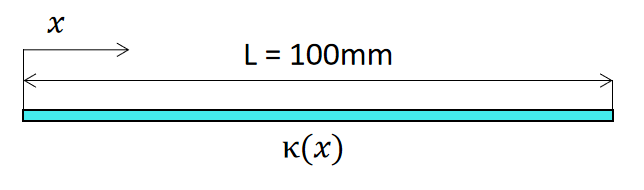
\includegraphics[width = 0.75\linewidth]{figures/fem_sketch.png}
	\caption{Visualisation of element that is modelled in one-dimension}
	\end{figure}
	The derivation started as a one-dimensional stationary heat conduction problem with the below equations as a starting point.
	\begin{equation}
	\label{heateq1}
	q_{,x}-f = 0  \text{  ...(1)} ; q = -\kappa u_{,x} \text{  ...(2)} 
	\end{equation}
	Integrating Equation \ref{heateq1} (1) over the length of the element(shown in Figure \ref{femfig}) and introducing a weighting function $w(x)$ we obtain \ref{heateq2}. 
	Since the derivative of $w(0)$ is known and $q_{,x}$ is unknown. 
	The first term in \ref{heateq2} is integrated by parts. 
	After the integration by parts and substituting $q$ with \ref{heateq1} (2) Equation \ref{heateq3} is created.
	\begin{equation}
	\label{heateq2}
	\int_{x=0}^L wq_{,x}dx - \int_{x=0}^L wfdx = 0
	\end{equation}
	\begin{equation}
	\label{heateq3}
	\int_{x=0}^L wku_{,x}dx + \int_{x=0}^L wfdx - \left.wq\right|_0^L = 0
	\end{equation}
	\subsection{Existing Model}
	For this project an existing finite element model of heat diffusion by Prof. N de Koker was modified for usage in the Bayes' theorem~\ref{bayes_eq}. 
	This model is used to determine the likelihood function. 
	The current model uses the standard Euro code $\kappa$-values as well as the specific heat specified in the \citep{Euro:2004}. 
	
	The model discretises the wooden element into 32 different elements. For finite element analysis, there are always more elements used to generate the model than usually evaluated. This is done to improve the accuracy of said model.
	The model is a one dimensional finite element model that takes time differentiation into account.
	
	\subsection{Adapted Model}	
	The model was changed into a function that takes $\kappa$-values and provides a new temperature distribution over the elements for the different $\kappa$-values. 
	This function is used in the posterior calculation to determine the likelihood function.
	

\section{Inversion method}
%here we will discuss everything that we did
The basis of the stochastic analysis is the adapted Bayesian equation \ref{modbayes} below. 
TODO: further interpret

\begin{equation}
\label{modbayes}
\pi^* (x|T) = \exp\left(-\frac{(\mu - x)^2}{2\sigma_{\mu}^2}\right) \cdot \exp\left(-\frac{\left(T-M(x)\right)^2}{2\sigma_{\text{temp}}^2}\right)
\end{equation}

	\subsection{Prior probability}
	
	\begin{equation}
	\label{prior}
	\pi(x) = \exp\left(-\frac{(\mu - x)^2}{2\sigma_{\mu}^2}\right)
	\end{equation}

	The prior probability function (Equation \ref{prior} ) is based on the $\kappa$-values assumed prior to any simulation or analysis. 
	The $\sigma_{\mu}$ in this equation was assumed to be equal to $0.13$ W/m$\cdot$K,
	In this case, the prior values are indicated as $\mu$ and refer to the vector of $\kappa$-values(\ref{euroK}) at specific temperatures ?TODO how to indicate?
	
	\begin{equation}
	\label{euroK}
	\mu =
		\begin{bmatrix}
		0.12\\ 
		0.12\\ 
		0.12\\ 
		0.12\\ 
		0.15\\ 
		0.07\\
		0.09\\ 
		0.35\\ 
		1.5\\
		\end{bmatrix}
	\end{equation}
	
The $x$ (in Equation \ref{prior}) refers to a vector of randomised $\kappa$-values that correspond with the same temperatures as the values in the $\mu$ vector.
The first iteration of randomised $\kappa$-values are generated by creating a random perturbation of the $\mu$ vector.
By multiplying the $\mu$ vector with $(0.5+\vec{\text{rand}})\cdot1.5)$ the first values of $x$ are guaranteed to be within an acceptable range of the prior values.
The process of obtaining the $x$ vector after the first iteration is discussed later in section \ref{mcmcexp}.


Initially the program was written to generate completely random new values for the first iteration of $x$. 
This later proved to not only be unnecessary, but also made the process less accurate as there was a larger burn-in period* before the values were anywhere near the actual solution.
To increase the accuracy and reduce the number of times the program needed to run to produce a sufficient number of accurate samples, the program was changed to the current method.
The prior function in this case was relatively easy to generate and incorporate into the program as a well defined list of prior values exists.

* explain and validate burn-in for machine learning (TODO)
	\subsection{Likelihood probability function}
		\begin{equation}
		\label{likelihoodfunc}
		\pi(T) = \exp\left(-\frac{\left(T-M(x)\right)^2}{2\sigma_{\text{temp}}^2}\right)
		\end{equation}
		
		The likelihood probability was more complex to implement, as this required utilisation of the function created from the finite element model as discussed in section \ref{femexpl}.
		This function will output the probability of the modelled values $M(x)$ given the measured temperature values ($T$).
		As can be seen in Equation \ref{likelihoodfunc}, the $M(x)$ vector is written as a function.
		The function indicated here takes the new randomised $x$ vector and then runs the model to provide a new temperature distribution over time at various nodes.
		The output of the finite element model was reduced such that only the nodes at the same depths as the thermocouples are provided to the likelihood function.
		For the likelihood function, the $\sigma_{\text{temp}}$ value was assumed to be 15$^{^\circ}$C.
		 

	\subsection{MCMC itegration}\label{mcmcexp}
	The two main parts of the MCMC integration (as mentioned in section \ref{tech}) are: how a value is deemed acceptable (Monte Carlo), and how the next random sample is selected after a previous sample is accepted (Markov Chain).
	
	To assist in choosing the next random sample, a step size that indicates how wide the range should be in which the next step will be found was chosen. 
	For this project a step size of $0.05$ W/m$\cdot$K was chosen.
	This concept can be visualized as follows: our accepted point(x1) is in the center of a cube. The next possible random point is randomly generate but still within the cube. 	
	After this next number is selected, the cube moves such that the new point(x2) is now the centre ,and so it continues.
	See Figure \ref{cubeexplfig} for clarification.
	The above example simplifies the concept, but this understanding can now be expanded.
	If every coordinate direction in the simple example is seen as a single entry into the $x$ vector, then the example has only three $\kappa$-values.
	There are however 10 values, so the imaginary cube in this situation is now ten-dimensional (don't worry, no attempt at drawing that will be made).
	Another level of complication can be added if it is taken into account that every point in the cube is no longer equally likely.
	A distribution within the cube can be chosen; in this case a log-normal distribution was chosen.
	The shape of the cube then warps into a stranger shape with points closer to the center being more likely choices and the edges being less likely.
	\begin{figure}
	
	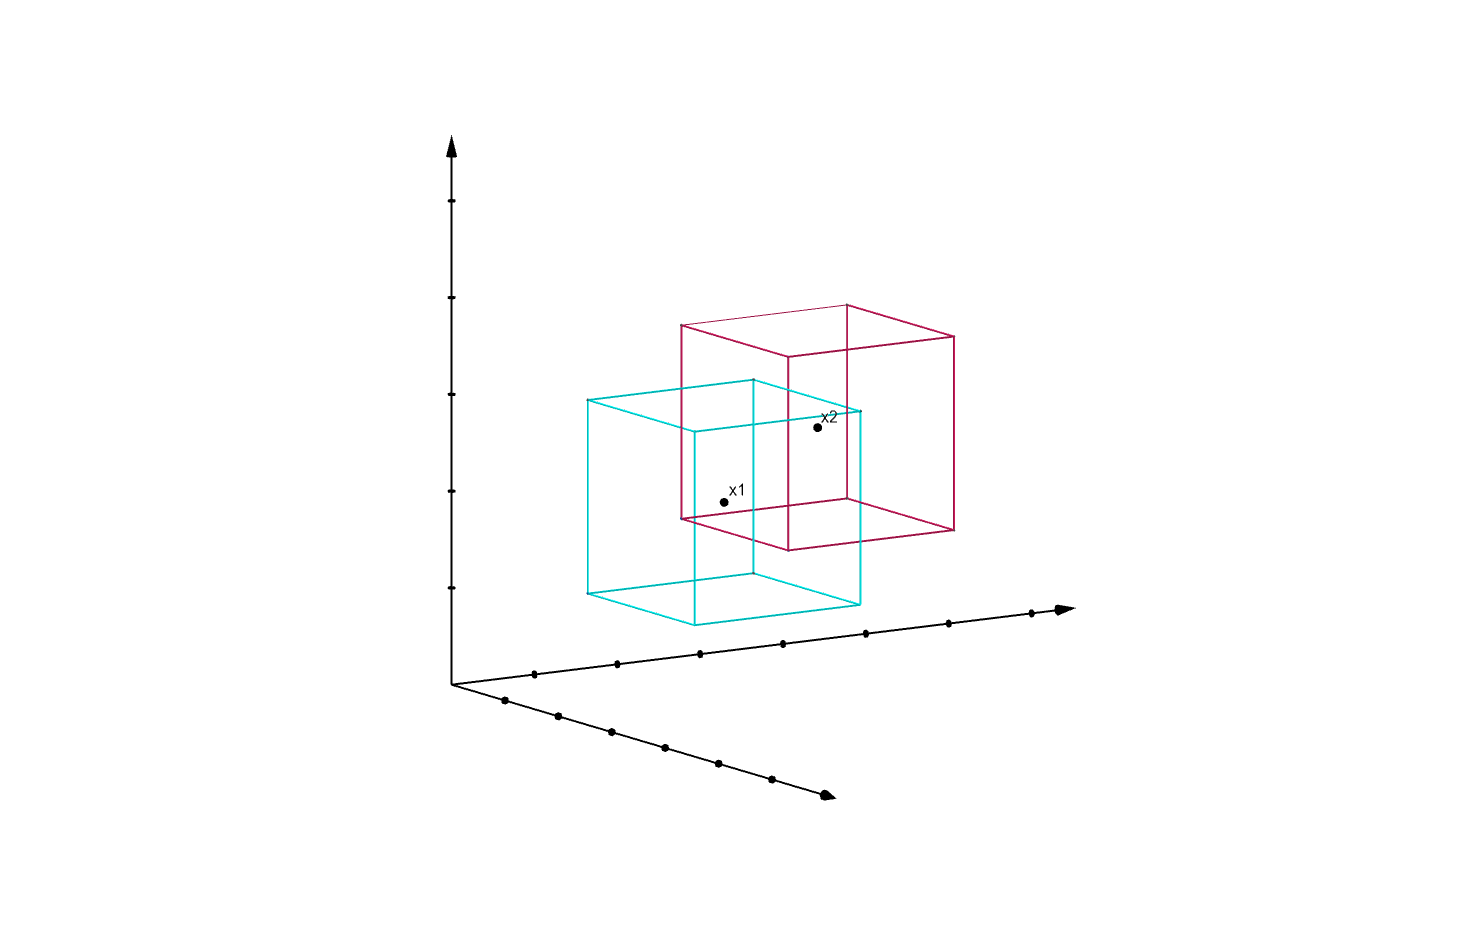
\includegraphics[width=\linewidth]{figures/MC_cubes.png}
	\caption{Three-dimensional example of Markov Chain application(Generated on \url{https://www.geogebra.org/3d})}
	\label{cubeexplfig}
	\end{figure}
	
	
	The acceptance criteria of the new $x$-vector is based on the proximity of the value to 
	
	
